\documentclass[10pt]{article}
\usepackage[utf8]{inputenc}
\usepackage{pgf,tikz}
\usetikzlibrary{arrows}
\pagestyle{empty}
\begin{document}
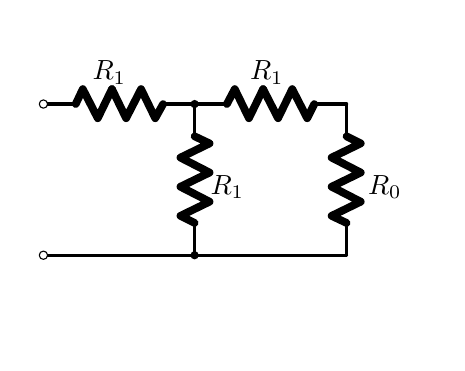
\begin{tikzpicture}[line cap=round,line join=round,>=triangle 45,x=1.0cm,y=1.0cm]
\clip(-0.2,0) rectangle (5,4);
\draw [line width=2.8pt] (0.87,3.22) -- (0.69,2.85) -- (0.5,3.22) -- (0.41,3.03);
\draw [line width=2.8pt] (0.87,3.22) -- (1.05,2.85) -- (1.24,3.22) -- (1.42,2.85) -- (1.52,3.03);
\draw [line width=2.8pt] (2.79,3.22) -- (2.61,2.85) -- (2.43,3.22) -- (2.33,3.03);
\draw [line width=2.8pt] (2.79,3.22) -- (2.98,2.85) -- (3.16,3.22) -- (3.35,2.85) -- (3.44,3.03);
\draw [line width=2.8pt] (3.85,1.52) -- (3.66,1.61) -- (4.03,1.79) -- (3.66,1.98) -- (4.03,2.16) -- (3.66,2.35) -- (4.03,2.53) -- (3.85,2.62);
\draw [line width=2.8pt] (1.92,1.52) -- (1.74,1.61) -- (2.11,1.79) -- (1.74,1.98) -- (2.11,2.16) -- (1.74,2.35) -- (2.11,2.53) -- (1.92,2.62);
\draw [line width=1.2pt] (0,3.03)-- (0.41,3.03);
\draw [line width=1.2pt] (1.52,3.03)-- (2.33,3.03);
\draw [line width=1.2pt] (1.92,3.03)-- (1.92,2.62);
\draw [line width=1.2pt] (1.92,1.52)-- (1.92,1.11);
\draw [line width=1.2pt] (1.92,1.11)-- (3.85,1.11);
\draw [line width=1.2pt] (3.85,1.11)-- (3.85,1.52);
\draw [line width=1.2pt] (3.85,2.62)-- (3.85,3.03);
\draw [line width=1.2pt] (3.85,3.03)-- (3.44,3.03);
\draw [line width=1.2pt] (1.92,1.11)-- (0,1.11);
\draw (0.5,3.7) node[anchor=north west] {$R_1$};
\draw (2.5,3.7) node[anchor=north west] {$R_1$};
\draw (2,2.25) node[anchor=north west] {$R_1$};
\draw (4,2.25) node[anchor=north west] {$R_0$};
\fill [color=white] (0,3.03) circle (1.5pt);
\draw [color=black] (0,3.03) circle (1.5pt);
\fill [color=black] (1.92,3.03) circle (1.5pt);
\fill [color=black] (1.92,1.11) circle (1.5pt);
\fill [color=white] (0,1.11) circle (1.5pt);
\draw [color=black] (0,1.11) circle (1.5pt);
\end{tikzpicture}
\end{document}